\section{توفر الذكاء الاصطناعي}
\label{sec:settings-feature-ai-availability}

تحدد هذه الصفحة أين يعمل الذكاء الاصطناعي في المؤسسة. وتسمي كل ميزة منه «مكاناً»، مثل مساعد الكتابة أو ملخص الإشعارات، ولكل مكان قرار مستقل. تفيدك الصفحة عندما تريد إيقاف ميزة لا تناسب عملكم، أو حصر ميزة في أعضاء محددين. يفتحها مالك المؤسسة أو من يحمل دور المسؤول على مستوى المؤسسة.

يتحدد وضع كل مكان بهذا الترتيب: قاعدة العضو أولاً، ثم قاعدة «الجميع»، ثم اختيار العضو نفسه. فإذا لم توجد قاعدة ولا اختيار، بقي المكان مفعّلاً. ويُستثنى «المساعد»؛ فهو متوقف حتى يشغّله مسؤول، ولا يشمل هذا الإعداد المساعد عبر واتساب.

\begin{rcnote}[مثال: شركة الأفق]
يترك مسؤول النظام مساعد الكتابة على «اختيار العضو» عند ①، ويبقي «المساعد» متوقفاً للجميع عند ②. ثم يضغط «تعديل القواعد» عند ④ أمام سارة الخطيب ويفعّل المساعد لها وحدها لتجربته قبل تعميمه.
\end{rcnote}

\begin{figure}[H]
\centering
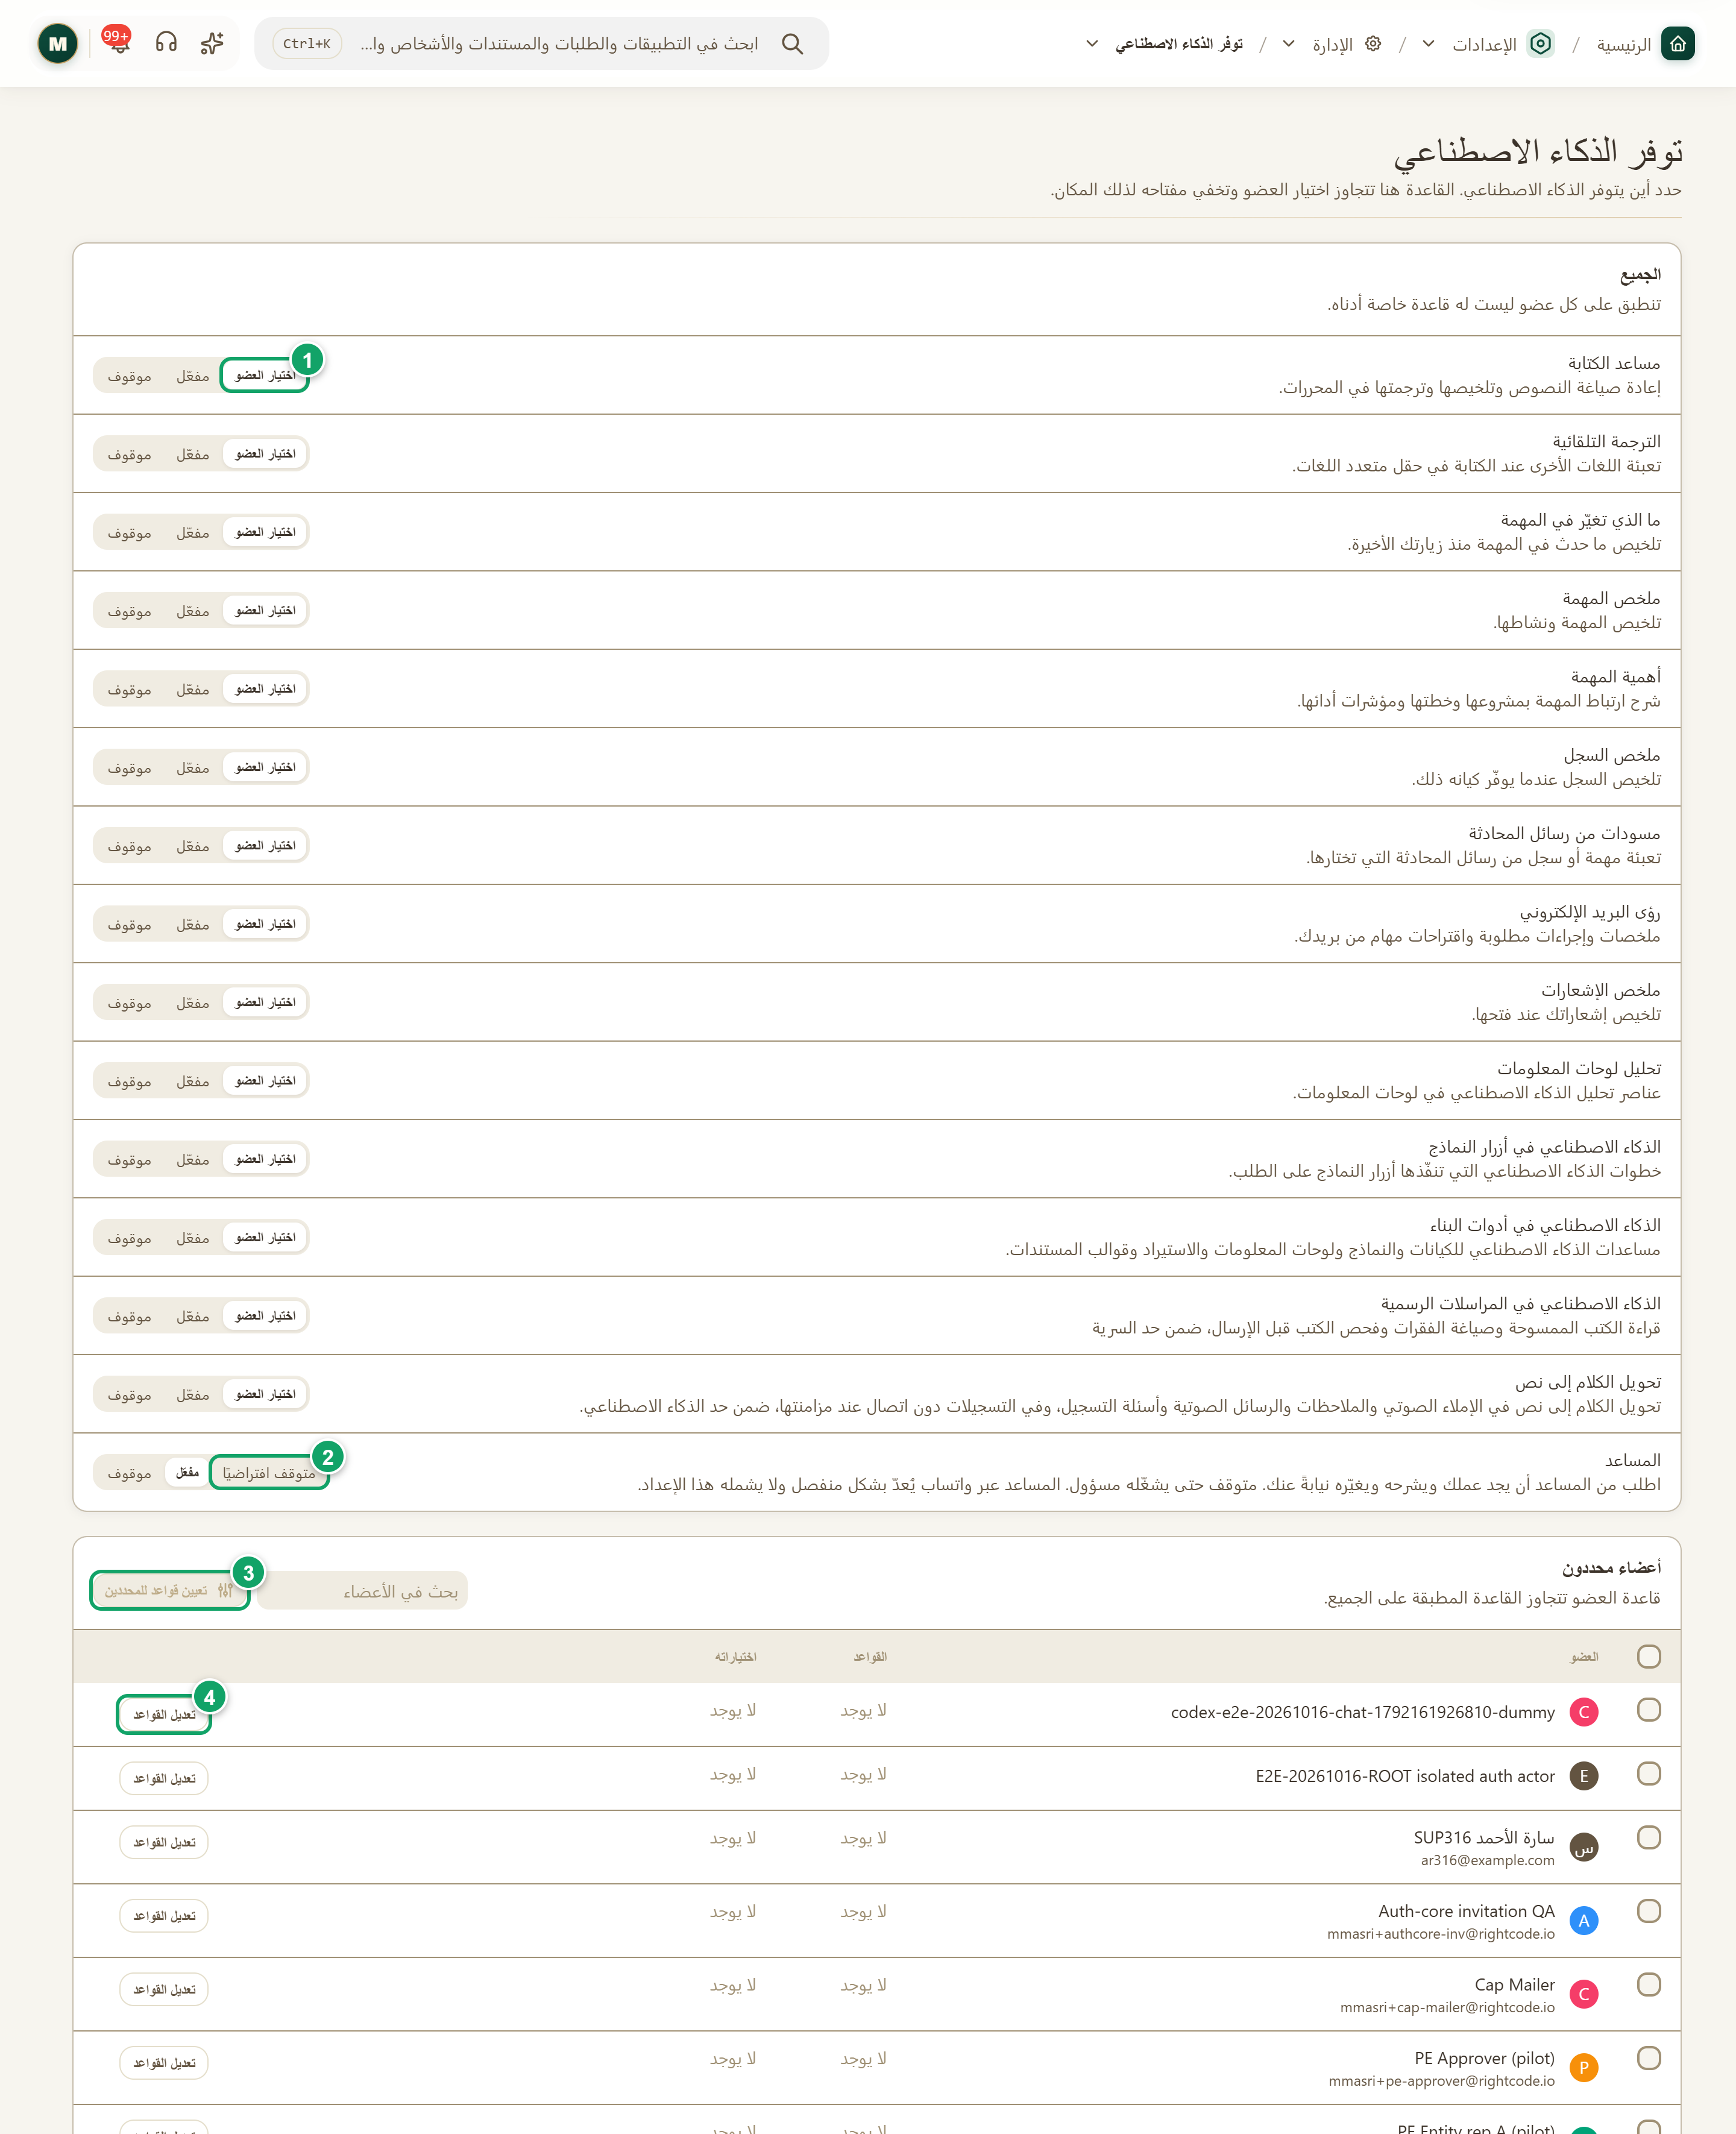
\includegraphics[width=0.95\linewidth,height=0.72\textheight,keepaspectratio]{figures/screens/ch08-ai-availability-ar.png}
\caption{قواعد الجميع والأعضاء المحددين}
\label{fig:settings-ai-availability-screen}
\shotnote{تجمع الصفحة كل أماكن الذكاء الاصطناعي في قائمة واحدة، وتحتها جدول الأعضاء الذين يمكن تخصيص قاعدة لهم. وتفيدك مقارنة عمود «القواعد» بعمود «اختياراته» في معرفة ما فرضه المسؤول وما اختاره العضو. ① «اختيار العضو»: يترك القرار للعضو، أما «مفعّل» و«موقوف» بجانبه فيفرضان القرار ويخفيان مفتاح العضو. ② «متوقف افتراضيًا»: خيار يحل في صف «المساعد» محل «اختيار العضو»، لأن العضو لا يقرر تشغيله، وقد اختارت مؤسسة الاختبار هنا «مفعّل». ③ «تعيين قواعد للمحددين»: يعمل بعد تحديد عضو أو أكثر في الجدول. ④ «تعديل القواعد»: لعضو واحد.}
\end{figure}

\begin{table}[H]
\centering
\caption{ماذا تقرر في هذه الصفحة؟}
\label{tab:settings-ai-availability-fields}
\begin{tabularx}{\linewidth}{R{4.2cm} Y}
\rcHeaderRow
\thh{القسم أو الخيار} & \thh{معناه}\\
«الجميع» & قاعدة لكل مكان تنطبق على كل عضو ليست له قاعدة خاصة. تُحفظ فور الضغط، ولا يوجد زر حفظ في هذا القسم.\\
«اختيار العضو» / «مفعّل» / «موقوف» & الخيار الأول يترك القرار للعضو في إعدادات حسابه. والخياران الآخران يقفلان المكان فيتجاهل النظام اختياره.\\
«أعضاء محددون» & قاعدة لعضو أو أكثر تتجاوز قاعدة «الجميع». تجد الأعضاء بالبحث بالاسم أو البريد الإلكتروني.\\
«القواعد» & الأماكن التي وضع لها المسؤول قاعدة لهذا العضو.\\
«اختياراته» & ما اختاره العضو بنفسه. يبقى محفوظاً حتى لو تجاوزته قاعدة، ويعود أثره عند إزالتها.\\
\end{tabularx}
\end{table}

\begin{figure}[H]
\centering
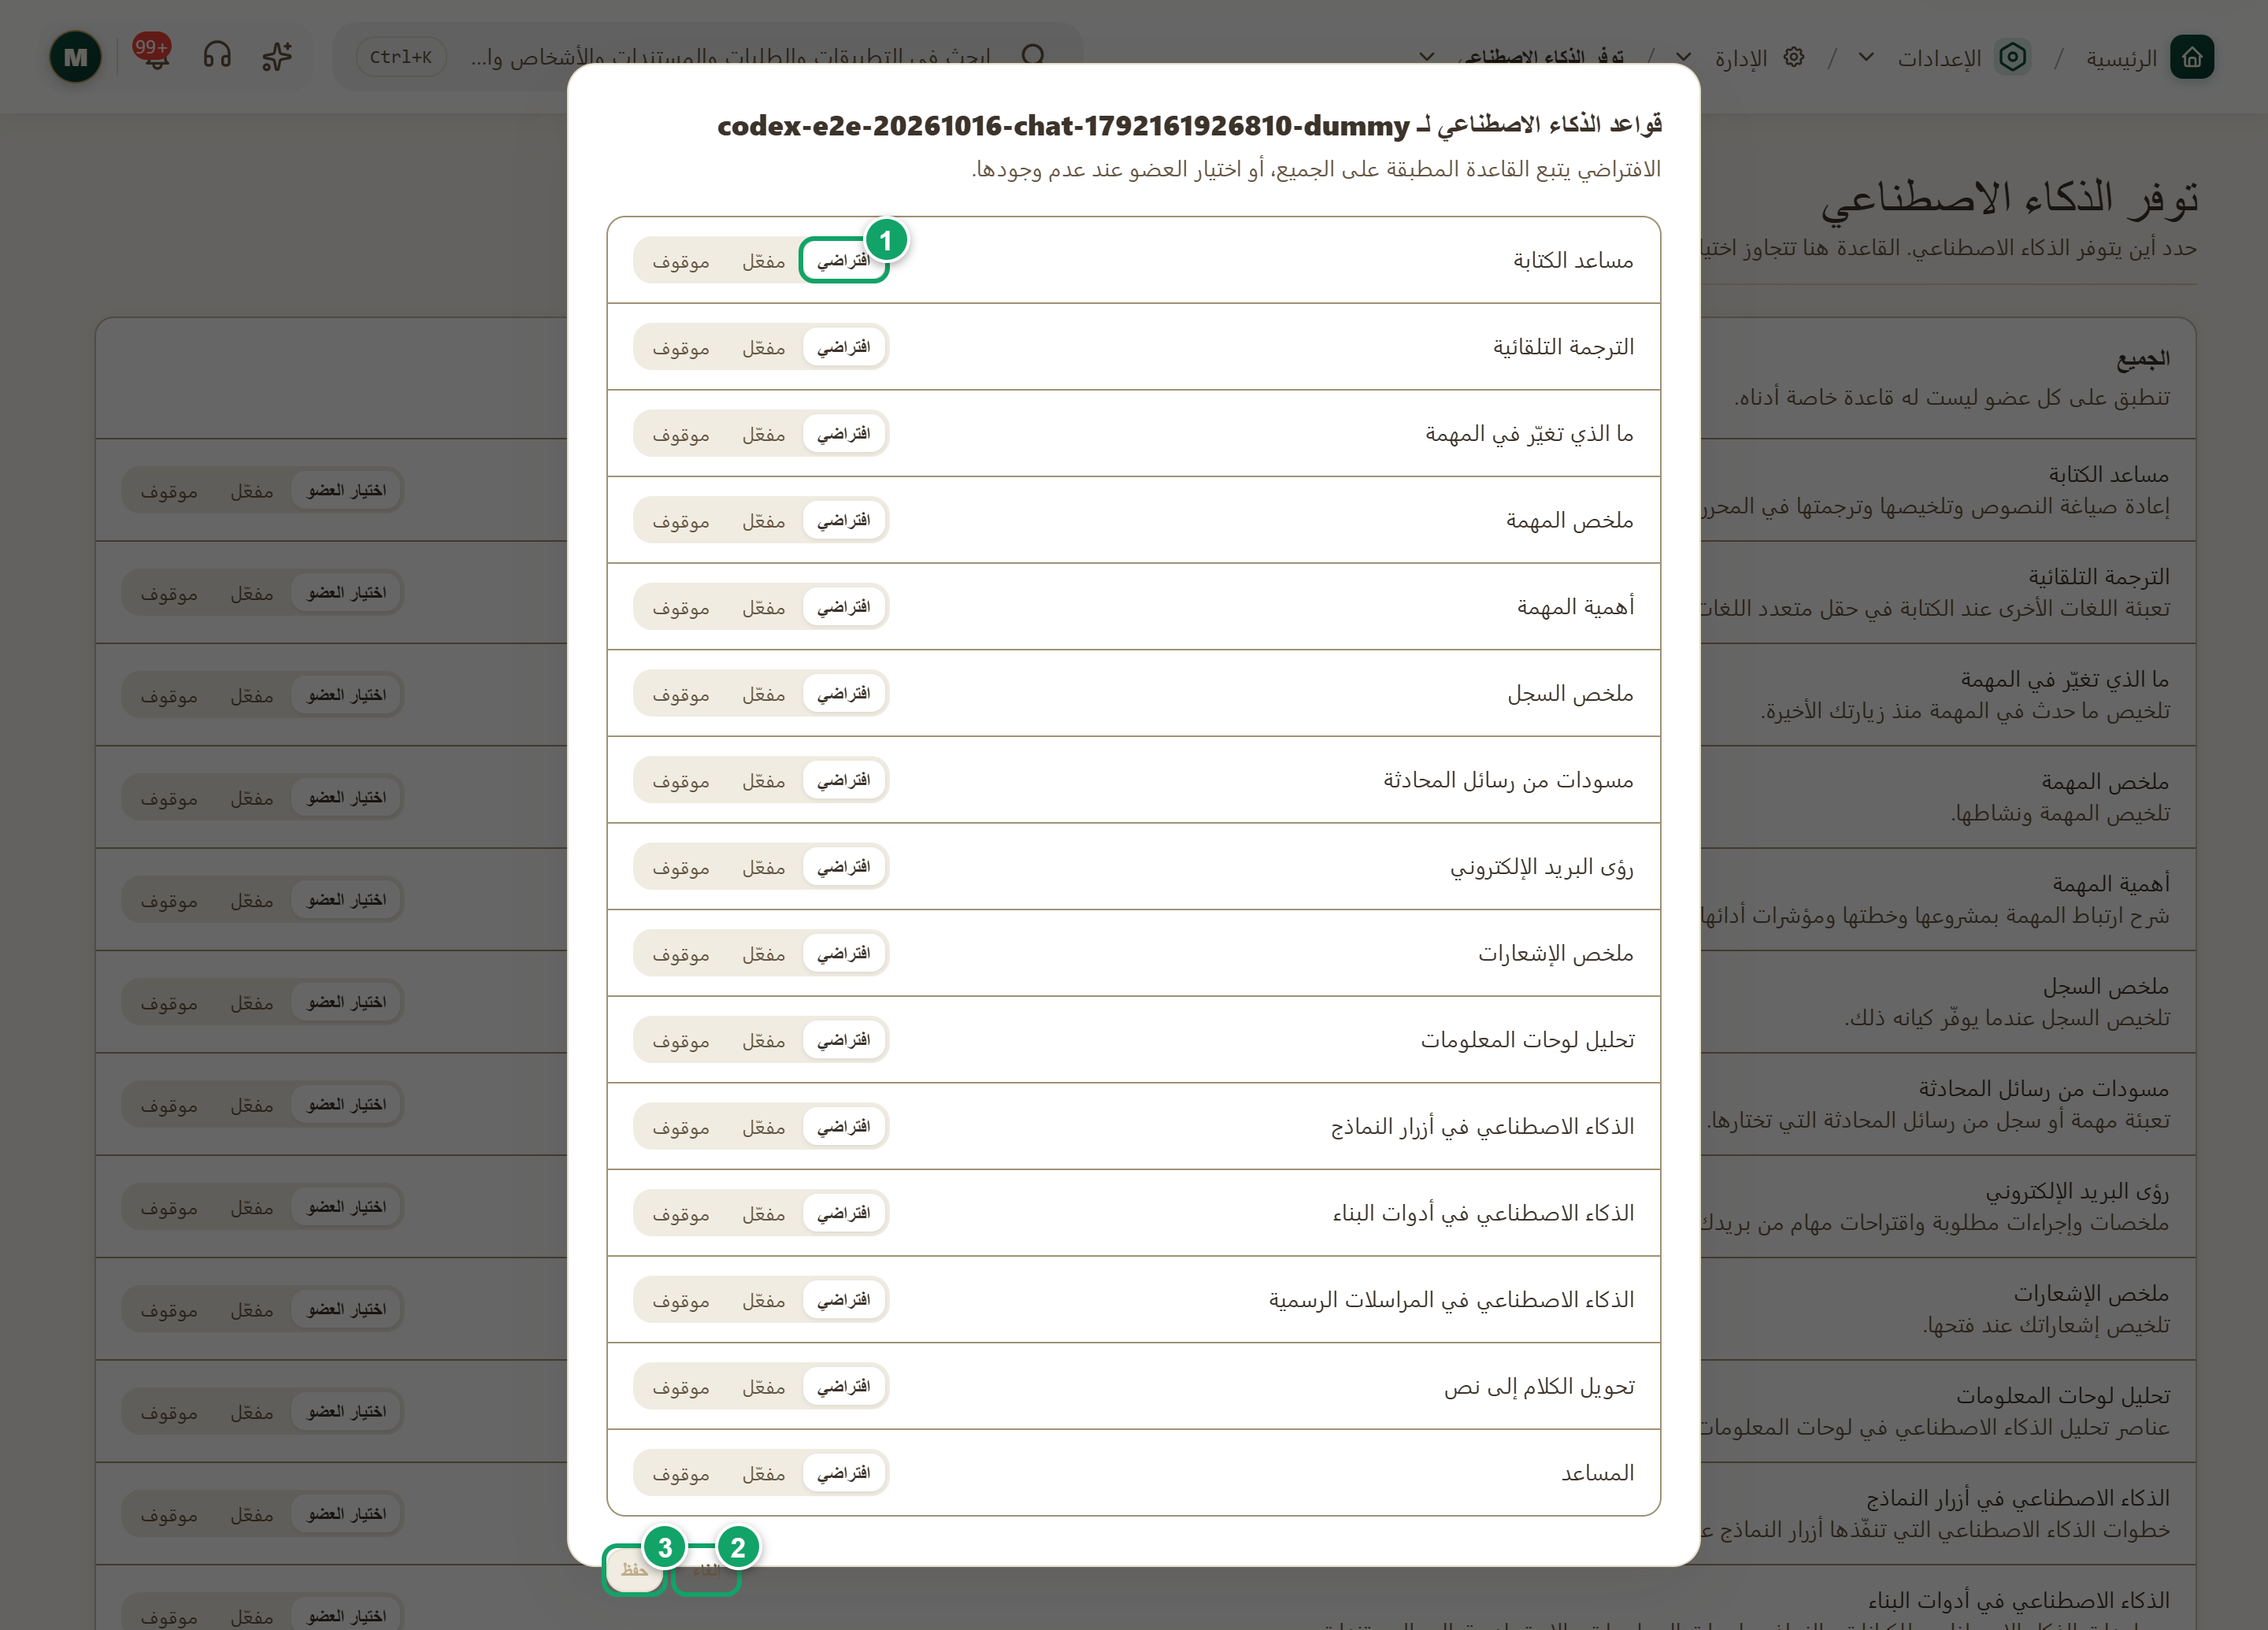
\includegraphics[width=0.95\linewidth,height=0.72\textheight,keepaspectratio]{figures/screens/ch08-ai-availability-member-ar.png}
\caption{قواعد الذكاء الاصطناعي لعضو}
\label{fig:settings-ai-availability-member-screen}
\shotnote{تعرض النافذة الأماكن نفسها، لكن لعضو واحد أو لمجموعة أعضاء محددين. وعند تحديد عدة أعضاء لا يتغير إلا المكان الذي عدّلته، فتبقى قواعدهم الأخرى كما هي. ① «افتراضي»: يتبع قاعدة «الجميع»، أو اختيار العضو عند عدم وجودها. ② «إلغاء»: يغلق النافذة دون تغيير. ③ «حفظ»: يبقى معطلاً حتى تغيّر قاعدة واحدة على الأقل.}
\end{figure}

\begin{enumerate}
\item افتح «الإعدادات» ثم «توفر الذكاء الاصطناعي».
\item اختر لكل مكان في قسم «الجميع» القيمة المناسبة. انتبه إلى أن الاختيار يُحفظ مباشرة.
\item لتخصيص عضو، اضغط «تعديل القواعد» في صفه. ولتخصيص عدة أعضاء، حدّدهم ثم اضغط «تعيين قواعد للمحددين».
\item اختر «مفعّل» أو «موقوف» للمكان المطلوب، ثم اضغط «حفظ».
\end{enumerate}

\textbf{تحقق:} تظهر رسالة «تم حفظ توفر الذكاء الاصطناعي.» ويعرض عمود «القواعد» المكان وحالته أمام العضو. وعندما يفتح العضو إعدادات حسابه لا يجد مفتاحاً لذلك المكان. إذا بقيت الميزة غائبة عن عضو رغم تفعيلها، فافحص قاعدته الخاصة أولاً لأنها تسبق قاعدة «الجميع»، ثم راجع صفحة «حدود الذكاء الاصطناعي».

\section{حدود الذكاء الاصطناعي}
\label{sec:settings-feature-ai-limits}

تضبط هذه الصفحة الميزانية التي يستهلكها الذكاء الاصطناعي، وتعرض ما استُهلك منها. فلكل طلب ذكاء اصطناعي كلفة تُسجل بالدولار الأمريكي، وتُخصم من حصة العضو إذا طلبه عضو، ومن «حصة المؤسسة بالكامل» إذا لم يرتبط بعضو. تفيدك الصفحة في منع تجاوز الميزانية، وفي معرفة الميزات الأعلى كلفة. يفتحها مالك المؤسسة أو من يحمل دور المسؤول على مستوى المؤسسة.

الحد مبلغ ثابت لا يتجدد تلقائياً كل شهر. فإذا رفعته أضيف الفرق إلى «المتبقي»، وإذا خفضته نقص منه الفرق. وعندما ينفد الرصيد يرفض النظام طلبات الذكاء الاصطناعي الجديدة من صاحب هذا الرصيد حتى يُرفع الحد.

\begin{rcnote}[مثال: شركة الأفق]
يلاحظ مسؤول النظام أن رصيد عمر حداد «منخفض»، فيبحث عن الميزة التي استهلكت الرصيد عند ②. ثم يحدد صف عمر في الجدول، ويكتب حداً جديداً عند ③، ويضغط «تطبيق الحد» عند ④.
\end{rcnote}

\begin{figure}[H]
\centering
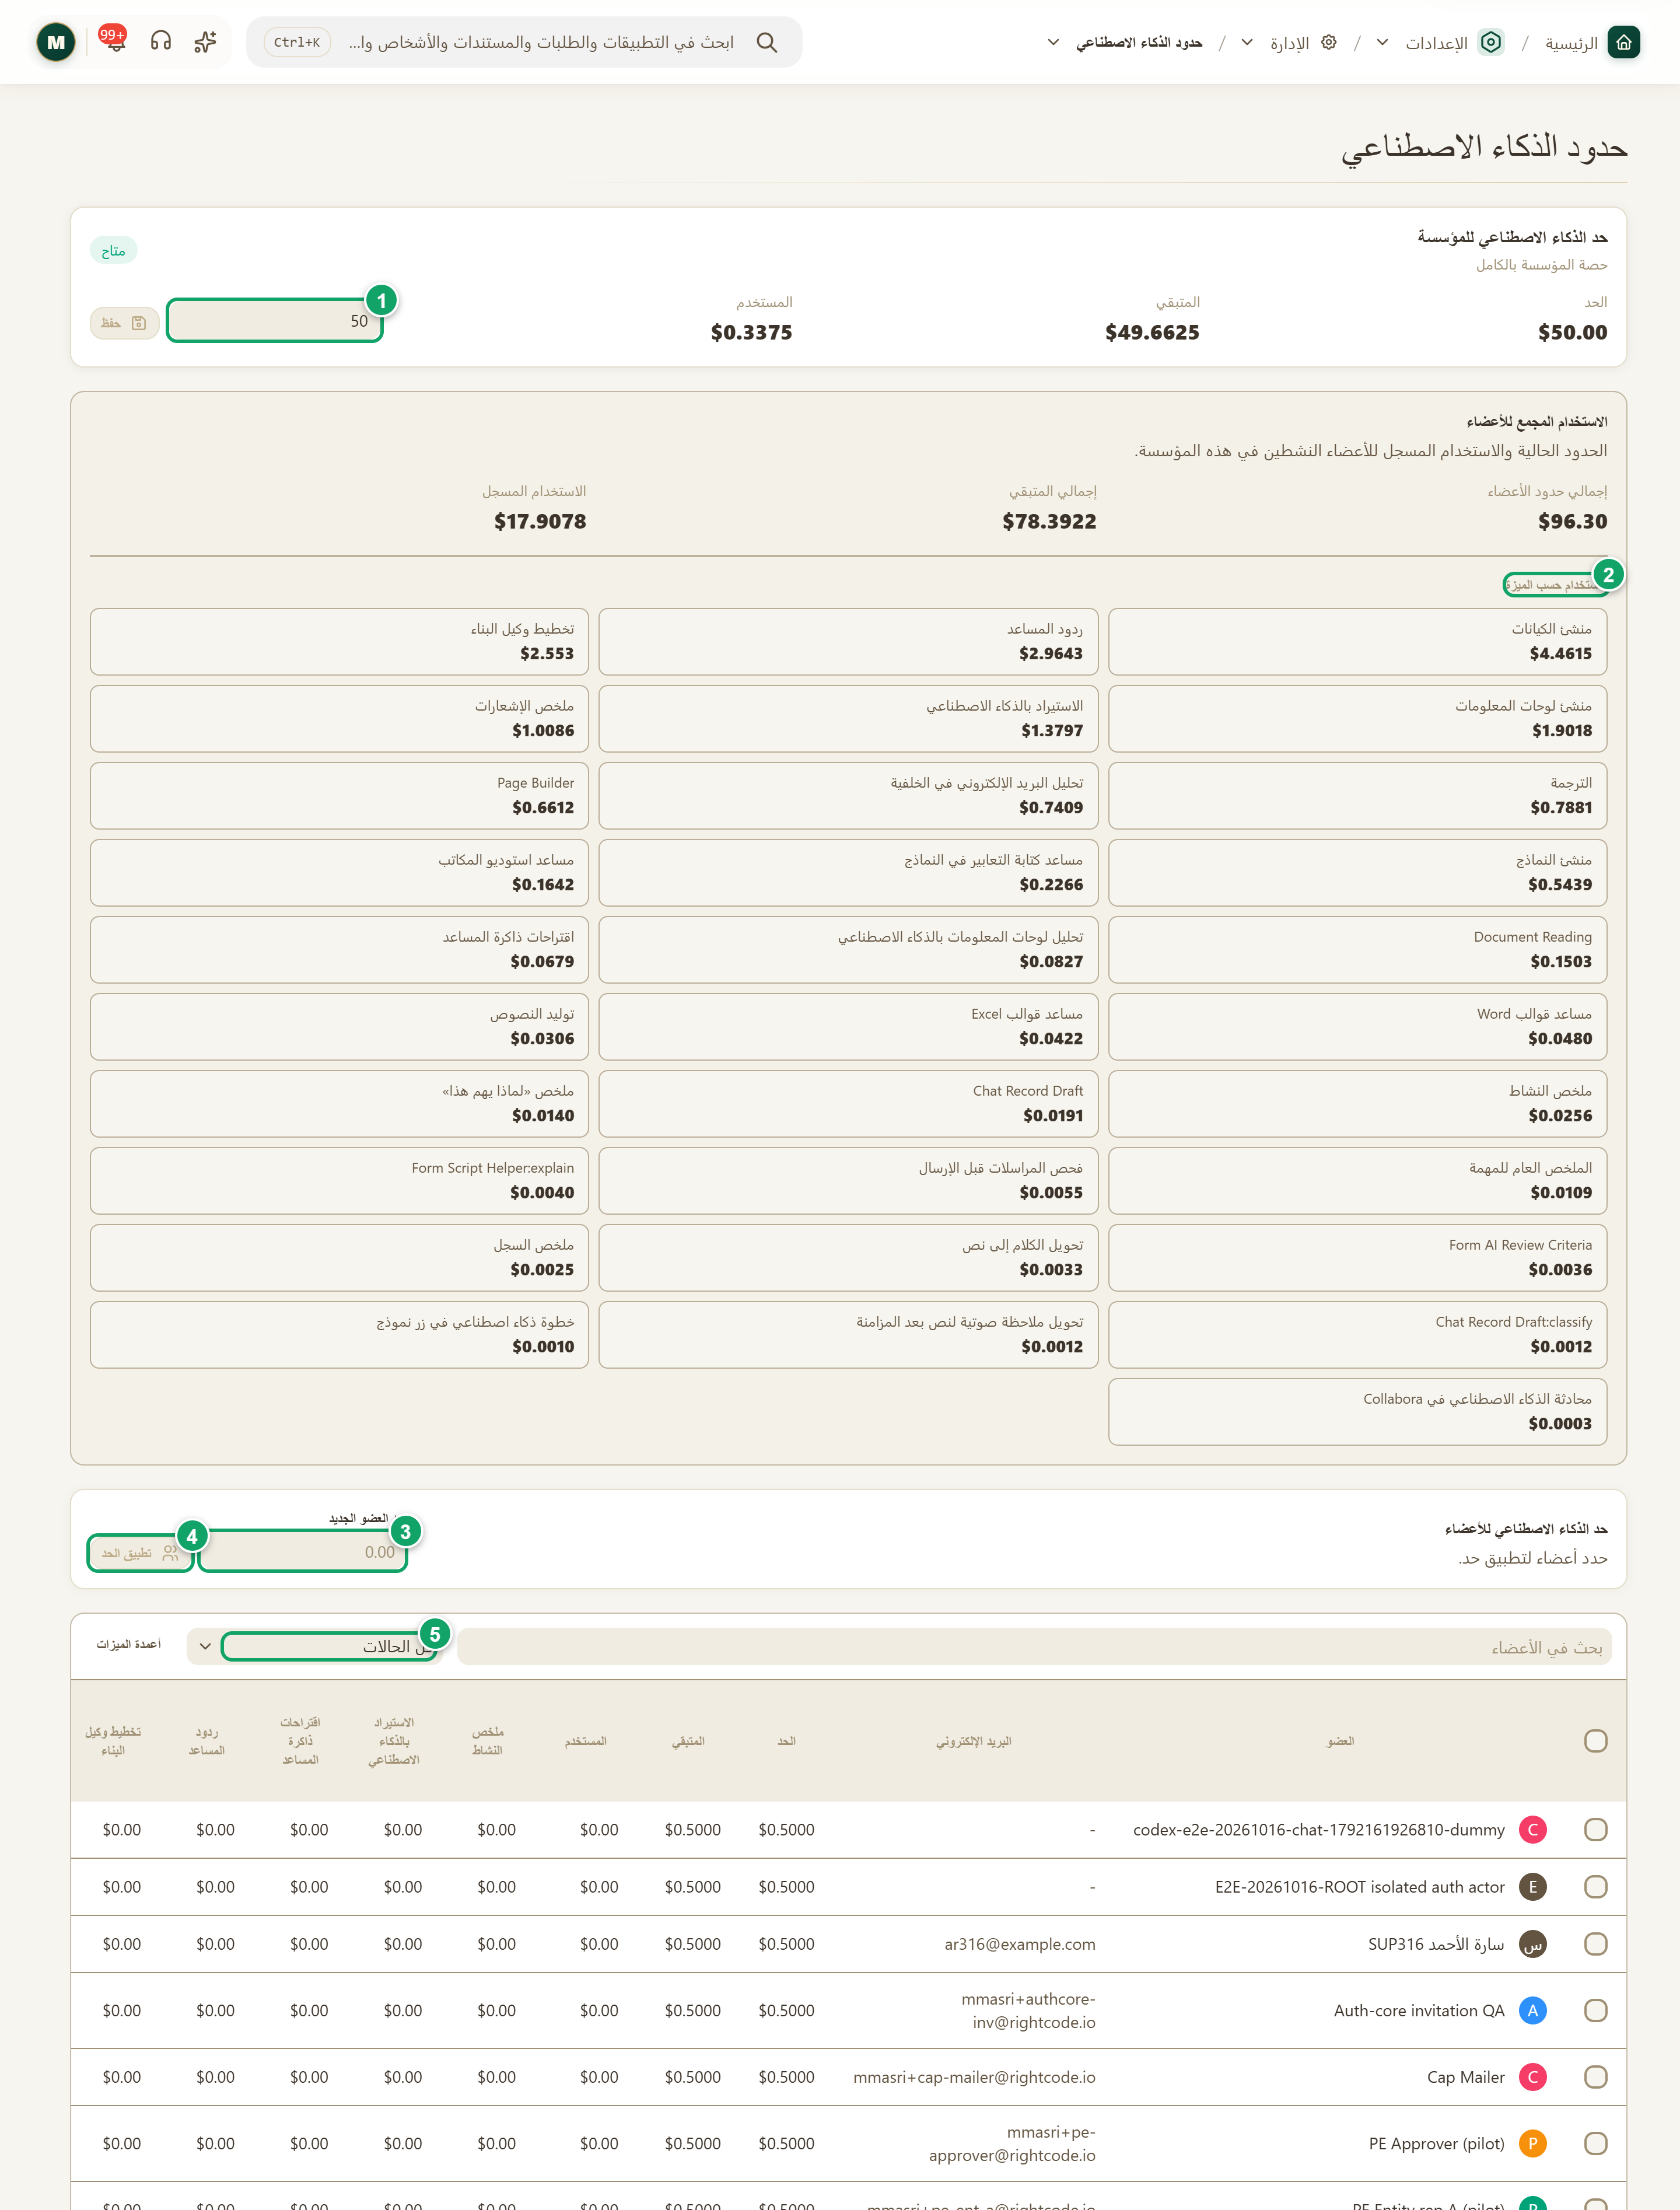
\includegraphics[width=0.95\linewidth,height=0.72\textheight,keepaspectratio]{figures/screens/ch08-ai-limits-ar.png}
\caption{حد المؤسسة وحدود الأعضاء والاستخدام}
\label{fig:settings-ai-limits-screen}
\shotnote{تعرض الصورة حصة المؤسسة، ثم مجموع حدود الأعضاء واستخدامهم، ثم جدولاً لكل عضو. والأرقام هنا لمؤسسة الاختبار. والفرق بين الجزأين مهم: تغيير حد المؤسسة لا يغيّر حدود الأعضاء، وتغيير حد عضو لا يمس حصة المؤسسة. ① حقل حد المؤسسة، ويُحفظ بزر «حفظ» بجانبه. ② «الاستخدام حسب الميزة»: يبيّن أين ذهبت الكلفة. ③ «حد العضو الجديد». ④ «تطبيق الحد»: يعمل بعد تحديد عضو وكتابة قيمة صحيحة. ⑤ «كل الحالات»: لتصفية الجدول بحالة الرصيد.}
\end{figure}

\begin{table}[H]
\centering
\caption{ماذا تقرأ وتسجل في هذه الصفحة؟}
\label{tab:settings-ai-limits-fields}
\begin{tabularx}{\linewidth}{R{4.2cm} Y}
\rcHeaderRow
\thh{القسم} & \thh{ما الذي يعرضه أو يسجله؟}\\
«حد الذكاء الاصطناعي للمؤسسة» & «الحد» و«المتبقي» و«المستخدم» لحصة المؤسسة، مع حقل لتغيير الحد.\\
«الاستخدام المجمع للأعضاء» & «إجمالي حدود الأعضاء» و«إجمالي المتبقي» و«الاستخدام المسجل» للأعضاء النشطين، ثم الكلفة لكل ميزة.\\
«حد الذكاء الاصطناعي للأعضاء» & حد واحد يُطبق دفعة واحدة على الأعضاء المحددين.\\
جدول الأعضاء & البريد والحد والمتبقي والمستخدم لكل عضو. ويضيف «أعمدة الميزات» كلفة كل ميزة.\\
«الحالة» & «متاح» عند توفر الرصيد، و«منخفض» إذا بقي أقل من 20\% من الحد، و«منتهٍ» عند نفاد الرصيد.\\
\end{tabularx}
\end{table}

\begin{enumerate}
\item افتح «الإعدادات» ثم «حدود الذكاء الاصطناعي».
\item لتغيير حصة المؤسسة، اكتب القيمة في حقل الحد ثم اضغط «حفظ».
\item لتغيير حد الأعضاء، حدّد صفوفهم في الجدول. يمكنك البحث أو التصفية بالحالة أولاً.
\item اكتب القيمة في «حد العضو الجديد»، ثم اضغط «تطبيق الحد».
\end{enumerate}

\textbf{تحقق:} تظهر رسالة «تم حفظ حدود الذكاء الاصطناعي.» ويتغير «الحد» و«المتبقي» في الصف نفسه بمقدار الفرق، وتتحدث «الحالة». ولا يقبل الحقل الأحرف ولا القيم السالبة؛ فإذا كتبتها ظهر بلون الخطأ ولم يُحفظ شيء.
